% 本文件是示例论文的一部分
% 论文的主文件是位于上级目录的 `main.tex`

\chapter{绪论}

\section{研究目的与意义}

在城市化进程加速和生活节奏日益加快的当下,外卖配送、即时出行等需求呈爆发式增长,
摩托车凭借其小巧灵活、通行便利的特性,在全球各地的城市交通体系中占据了愈发重要的地位。
无论是穿梭于大街小巷的外卖骑手,还是追求通勤效率的上班族,都将摩托车视为短途出行的优质选择。
这一市场需求的增长,有力推动了摩托车产业的蓬勃发展,其保有量在全国范围内持续攀升。\ref{fig:traffic}展示了某城市道路上摩托车驾乘人员的头盔佩戴情况。

随着摩托车数量的急剧增长,涉及摩托车的交通事故也逐渐增多。头盔作为摩托车驾乘人员唯一的保护装置,能够极大减少交通事故给驾乘人员带来的伤害,尽可能地保护驾驶员和乘客的生命安全\cite{hss}。尽管国家出台了强制佩戴头盔的交通法规
来保障骑行者的生命安全,但部分骑行者安全意识淡薄,依旧心存侥幸,不佩戴头盔就上路行驶。

当前,针对摩托车驾乘人员头盔佩戴情况的监管,主要依赖交警人工检查。然而,我国道路系统错综复杂,
交通流量庞大且情况瞬息万变,交警在维持交通秩序的同时,还要负责检查头盔佩戴情况,
工作负担极为沉重。人工检查不仅效率低下、耗费大量人力物力,而且在复杂路况和密集车流中,
极易出现漏检现象,难以确保监管工作的全面性和准确性。因此,一个摩托车驾乘人员头盔佩戴检测系统对减少人工工作量、提升检测速度和准确度有很大的意义。

\begin{figure}[!htb]
  \centering
  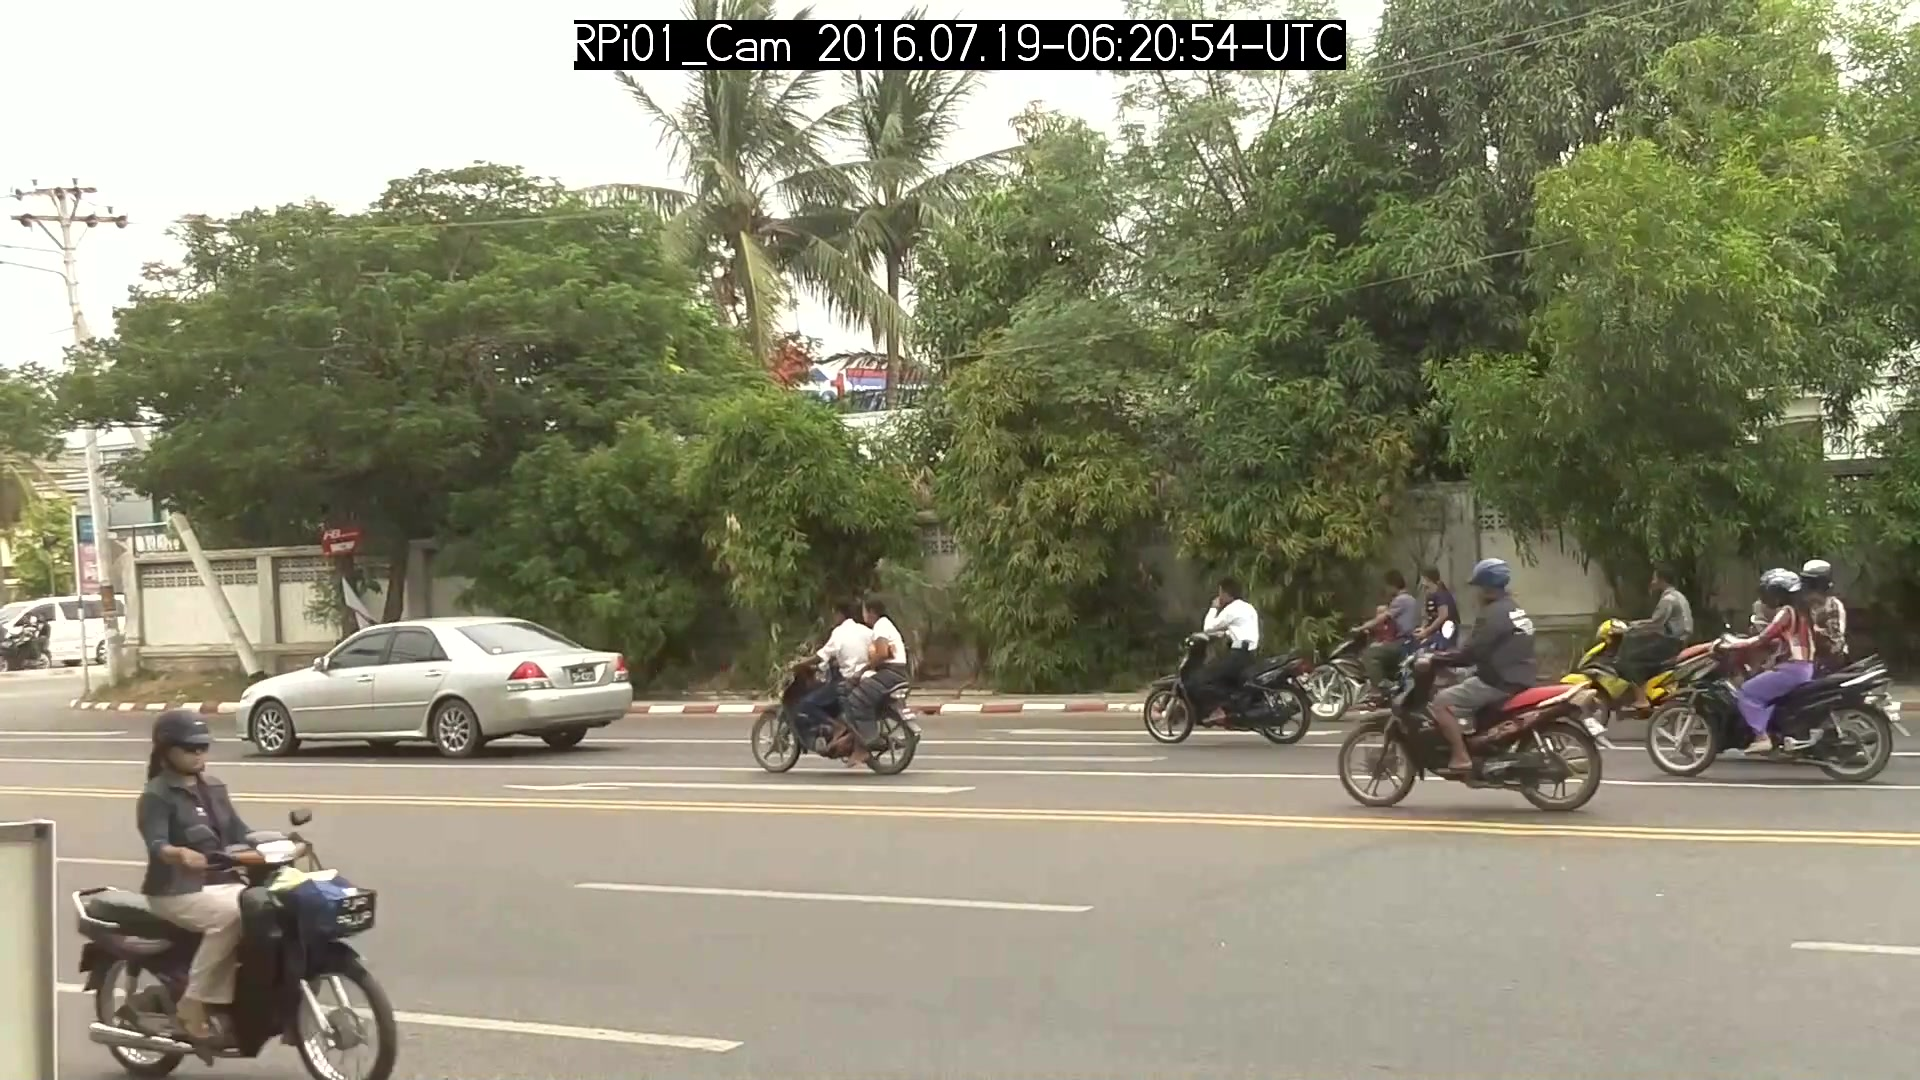
\includegraphics[width=0.85\textwidth]{figs/chap01/traffic}
  \caption{城市道路上摩托车驾乘人员头盔佩戴情况}
  \label{fig:traffic}
\end{figure}

本文基于YOLOv11目标识别算法,训练了能够检测头盔佩戴情况的模型,该模型能够实时识别图片或视频中摩托车驾乘人员是否佩戴头盔。此外,通过Vue和SpringBoot框架搭建系统,为用户提供图形界面化的操作平台,将检测结果持久化到数据库,以便后续查询历史检测记录以及进行数据的可视化。

\section{目标检测发展历程}

目标检测是计算机视觉领域的核心任务之一,它的发展历程如\ref{fig:his}所示。

\begin{figure}[!htb]
  \centering
  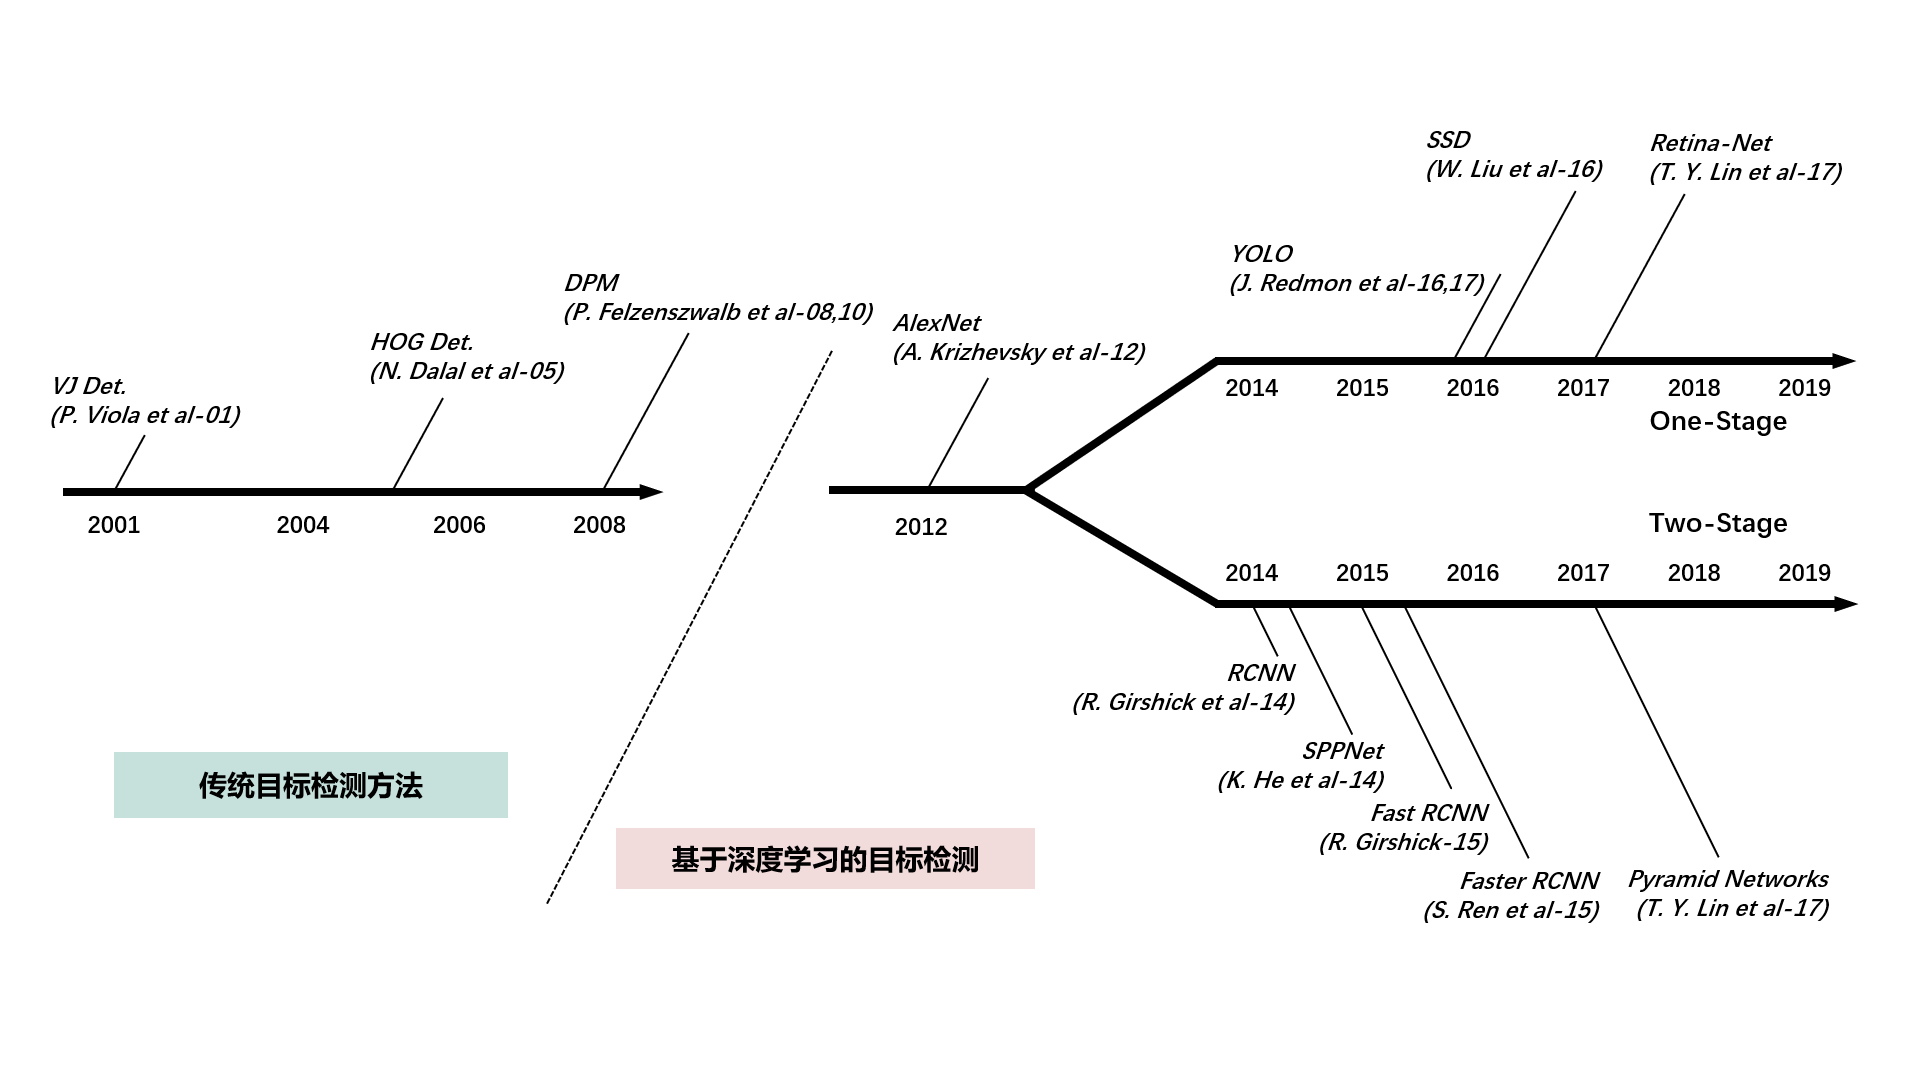
\includegraphics[width=0.9\textwidth]{figs/chap01/his.png}
  \caption{目标检测算法发展历程}
  \label{fig:his}
\end{figure}

\subsection{传统目标检测}
在深度学习兴起之前,目标检测算法高度依赖人工设计特征。受限于图像表示能力,研究者们需要设计复杂的特征表示。这一时期的代表成果深刻影响了后续目标检测技术的发展。

2001年,\textcite{Viola2001}首次在通用场景下实现了无约束的人脸实时检测。相较于同期算法,Viola-Jones(VJ)检测器在保持同等检测精度的前提下,运算速度实现了数十倍乃至数百倍的提升。该检测器运用滑动窗口,对图像内所有尺寸所有位置的窗口进行遍历,判别窗口中是否存在人脸。VJ检测器融合了“积分图像”、“特征选择”以及 “检测级联”技术,大幅提升了检测效率。

Dalal与Triggs于2005年提出方向梯度直方图(HOG)描述器,对当时的尺度不变特征变换和形状语境做出重要改进\cite{Dalal2005}。HOG描述器被设计为在密集的均匀间隔单元网格(区块)上计算,并使用重叠局部对比度归一化方法来提高精度。HOG描述器的主要目标是行人检测,如若要检测不同大小的对象,则需要让HOG检测器在保持检测窗口大小不变的情况下,对输入图像进行多次重设尺寸。

DPM(Deformable Part Models)在目标检测领域具有重要地位,该模型最早由P. Felzenszwalb在2008年提出\cite{Felzenszwalb2008},作为 HOG 检测器的延伸版本,后续经R. Girshick等人不断优化改进\cite{Felzenszwalb2010Cascade}。DPM采用“分而治之”的思想,通过检测对象的各个部件实现目标识别。

\subsection{基于深度学习的目标检测}
2012年,\textcite{alexNet}提出了一种经典的卷积神经网络,在ImageNet大规模视觉识别挑战赛中以压倒性优势刷新了记录,它的出现对深度学习发展具有里程碑式的意义。基于深度学习的目标检测算法主要分两类:基于回归的One-Stage与基于候选区域的Two-Stage。

\subsubsection{R-CNN系列算法}
2014年,\textcite{rcnn}提出的R-CNN的思路为:首先通过选择性搜索\cite{selectSearch}算法来提取可能包含目标的候选框,并将候选框调整成固定大小,然后通过AlexNet进行特征提取,最后利用SVM分类器识别每个区域内的目标。尽管R-CNN在目标检测领域实现了突破性进展,但其局限性也较为突出。该模型需对数量众多且相互重叠的候选区域(单张图像通常生成超过2000个候选框)进行特征提取计算,检测速度极慢。同年,\textcite{sppnet}通过引入空间金字塔池化层(SPP),突破了传统CNN需要固定输入尺寸的约束,实现对任意尺寸图像生成固定长度特征表示,将检测速度提升至R-CNN的20倍以上。

2015年,\textcite{fast-rcnn}提出Fast R-CNN检测器,作为对R-CNN和SPPNet的进阶优化成果,其创新地实现了在同一网络配置下同步训练检测器与边界框回归器,降低了训练和推理时间,大大提升了模型的性能。

\textcite{faster-rcnn}提出的Faster R-CNN检测器是第一个端到端的,也是第一个接近实时的深度学习检测器。它引入了RPN(Region Proposal Network)来提升检测速度和性能。RPN用于自动生成候选区域,在性能上要比选择性搜索算法好很多,推动目标检测系统从分散模块逐步整合为统一的端到端学习架构。


\subsubsection{YOLO系列算法}
2016年,\textcite{yolo}提出的YOLO算法,是One-Stage算法及YOLO系列的开山之作。其核心机制是利用单个卷积神经网络对整幅图像进行处理,将图像分割为多个区域后,直接预测各区域的边界框与对应类别概率,并通过概率加权对边界框进行筛选,经阈值处理后输出高置信度检测结果。YOLOv1将输入图像划分为nxn网格,每个网格单元负责预测内部目标的边界框及类别信息,每个边界框均附带基于交并比(IOU)计算的置信度分数,用于评估框内存在目标的可能性。

在YOLOv1问世一年后,YOLOv2应运而生\cite{yolov2}。该模型因能够检测超过9000个不同对象,也被称作YOLO9000。YOLOv2的核心是提出了一种独特的联合训练算法,该算法能够同时利用检测数据与分类数据对目标检测器进行训练。通过标记检测图像学习目标精确定位,借助分类图像扩展模型识别类别范围、增强鲁棒性。

YOLOv3通过多尺度预测架构(三尺度特征金字塔)优化跨尺寸目标检测,并引入Darknet-53骨干网络,在COCO数据集上实现精度-速度双优平衡\cite{yolov3}。其采用独立Logistic分类器替代Softmax,支持多标签分类,同时修正了YOLOv2的底层数据加载缺陷。

2020年,YOLOv4的主干网络采用CSPDarknet53骨干网络,融合了跨阶段局部连接(CSPNet)策略。颈部网络集成改进型空间金字塔池化(SPP)与路径聚合网络(PAN),实现多尺度特征融合与跨层级信息增强\cite{yolov4}。YOLOv5采用基于PyTorch的模块化架构重构检测框架,在提升了速度和精度的同时,使网络结构更加轻量级。

YOLOv6是YOLO系列中的一次重大演变,由美团视觉团队开发\cite{yolov6}。YOLOv6通过硬件感知架构设计与动态训练策略的协同创新,在速度精度平衡与部署效率层面实现了突破性进展。其核心架构采用EfficientRep主干网络,基于RepVGG重参数化思想构建分层模块化结构,显著提升GPU推理效率;特征融合模块则重构为Rep-PAN拓扑,通过重参数化卷积增强跨尺度信息流,并结合解耦式预测头缩减冗余计算。同年提出的YOLOv7通过架构创新与动态训练机制的协同设计,在实时性与检测精度间实现突破性平衡\cite{yolov7}。其采用E-ELAN扩展型主干网络,通过多分支深度扩展与特征通道重组增强多尺度表征能力。YOLOv8是YOLO系列实时对象检测器的迭代版本,在准确性和速度方面提供尖端性能。YOLOv8由Ultralytics开发,引入了新功能和优化,使其成为各种应用中各种对象检测任务的理想选择。

2024年提出的YOLOv9通过可编程梯度信息(PGI)重构梯度传播路径,利用辅助可逆分支生成可靠梯度,结合广义高效层聚合网络(GELAN)融合CSPNet与ELAN架构优势,显著缓解深度网络的信息衰减问题\cite{yolov9}。同年提出的YOLOv10通过一致双分配策略实现无NMS训练,提升性能和推理效率;采用整体效率-精度驱动的模型设计策略,全面优化模型组件,降低计算开销、增强模型能力\cite{yolov10}。同年晚些时候的YOLOv11进一步革新特征提取机制,引入C3k2轻量化卷积块替代传统C2f结构;并设计C2PSA跨阶段空间注意力模块强化遮挡与小目标检测能力,成为迄今最高效的YOLO迭代版本。YOLOv11的网络架构将在下一章进行详细介绍。




% 2012 年,AlexNet的提出推动了深度学习在目标识别领域的广泛应用\cite{alexNet}。随后,R - CNN 系列\cite{rcnn}、
% Fast R - CNN\cite{fast-rcnn}、Faster R - CNN\cite{faster-rcnn} 等两阶段检测方法不断改进,显著提升了检测精度和效率。SSD 
% 和 YOLO 系列作为单阶段检测方法,以不同的方式实现了高效的目标检测。其中,YOLO 系列将
% 目标检测转化为回归问题,极大地提高了检测速度,并且后续版本不断优化,加入了多尺度训练等技术,
% 以应对不同尺寸物体的检测需求。

\section{YOLO在交通安全领域的应用}
YOLO(You Only Look Once)是一系列目标检测算法,它基于深度学习技术,将目标检测问题转化为
回归问题进行处理,这一独特的设计思路使得它在速度和精度方面都取得了很好的平衡,在交通安全领域得到了非常广泛的实际应用。

2025年,张浩晨等人基于YOLOv8算法,首先提出了结合Transformer结构全局特征提取能力的模块C2Former代替C2f模块,设计了重感知的门控线性单元GRMLP优化Transformer分支非线性表达能力,提升了在小目标、遮挡目标等场景下对交通车辆检测的精度\cite{ex1}。肖振久等人设计动态特征融合网络,利用多样化卷积和通道缩放降低模型复杂度,并结合SPDConv重构颈部网络,增强小目标边缘信息提取的能力,在平衡检测精度的前提下提出了DEL–YOLO轻量化安全帽佩戴检测算法\cite{ex2}。\textcite{ex3}针对雾天场景下的车辆检测需求,基于DAWN和FD数据集构建四类车辆标注,并对比了YOLO-V5/V8系列模型的性能。通过引入注意力模块(CBAM、NAM、SimAM)和BiFPN结构优化YOLO-V5s/V5l,优化了算法在雾天中对车辆的检测性能。

YOLO算法凭借其高效性与准确性,已在交通、工业、医疗等多个领域发挥其作用,提供了精准的实时监测能力,推动各个行业的智能化发展。

\section{研究与设计内容}

本文基于YOLOv11算法设计并实现了摩托车驾乘人员头盔佩戴检测系统,主要涉及模型训练、系统开发两个任务。

在模型训练这里,做了两方面工作。一方面,在数据标注环节,进行了细致且全面的处理。针对不同情况设置了多种标签,例如单一驾驶人佩戴、单一驾驶人未佩戴、驾驶员佩戴一位乘客未佩戴、驾驶员佩戴一位乘客佩戴等,并没有简单地将所有情况划分为佩戴和不佩戴两种,这样在检测时能为用户提供更详细的信息,让用户清楚了解当前驾驶人及乘客各自的头盔佩戴状况。另一方面,训练了两个关键模型,一个用于识别摩托车及驾乘人员整体头盔佩戴情况,另一个用于识别摩托车驾驶人员是谁。在训练过程中,使用YOLOv11n、YOLOv11s、YOLOv11m等不同模型进行尝试,并通过调整训练epoch来优化模型精度。

系统基于BS架构开发。B端页面为用户提供了两个操作页面,一个是用于上传图片或视频以请求检测的页面,用户可通过该页面发起检测需求;另一个是数据查询页面,用户能从该页面向服务端数据库发送历史检测结果查询请求,还可以对驾驶人、记录时间、记录地点等字段进行过滤。查询得到的结果会以柱状图、折线图等可视化的形式在页面呈现,为后续制定执法策略提供数据支持。S端负责处理B端页面传来的请求,当接收到用户上传的图片或视频后,先利用第一个模型预测图片中的头盔佩戴情况,之后对目标区域进行裁剪,再使用第二个模型检测目标区域的驾驶人员,最后将检测结果保存到数据库中。\ref{fig:source}和\ref{fig:result}表示了输入图片和检测结果。

\begin{figure}[!htb]
  \centering
  \begin{minipage}{0.45\textwidth} % 调整宽度以适应需求,两张图总宽度接近1
      \centering
      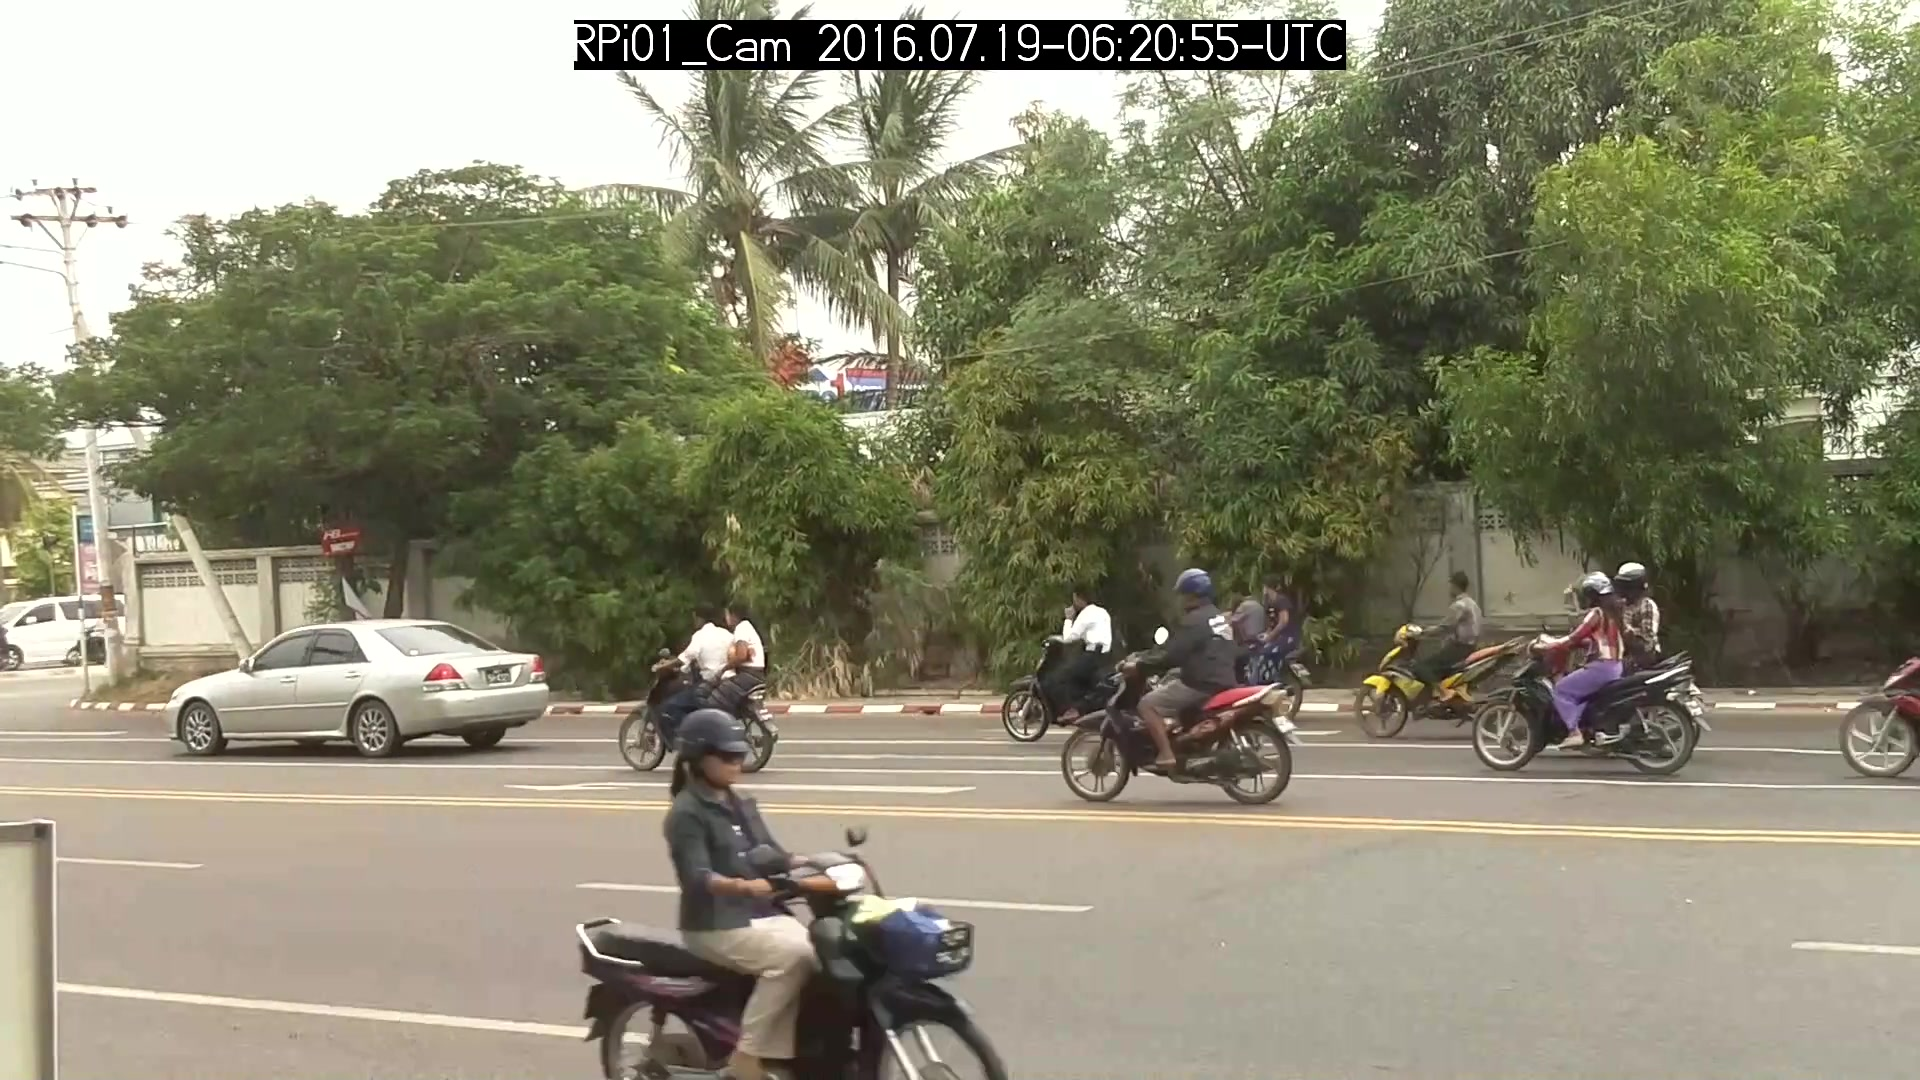
\includegraphics[width=\textwidth]{figs/chap01/source.jpg}
      \caption{选择图片}
      \label{fig:source}
  \end{minipage}
  \hfill % 使两张图片之间保持一定距离
  \begin{minipage}{0.45\textwidth}
      \centering
      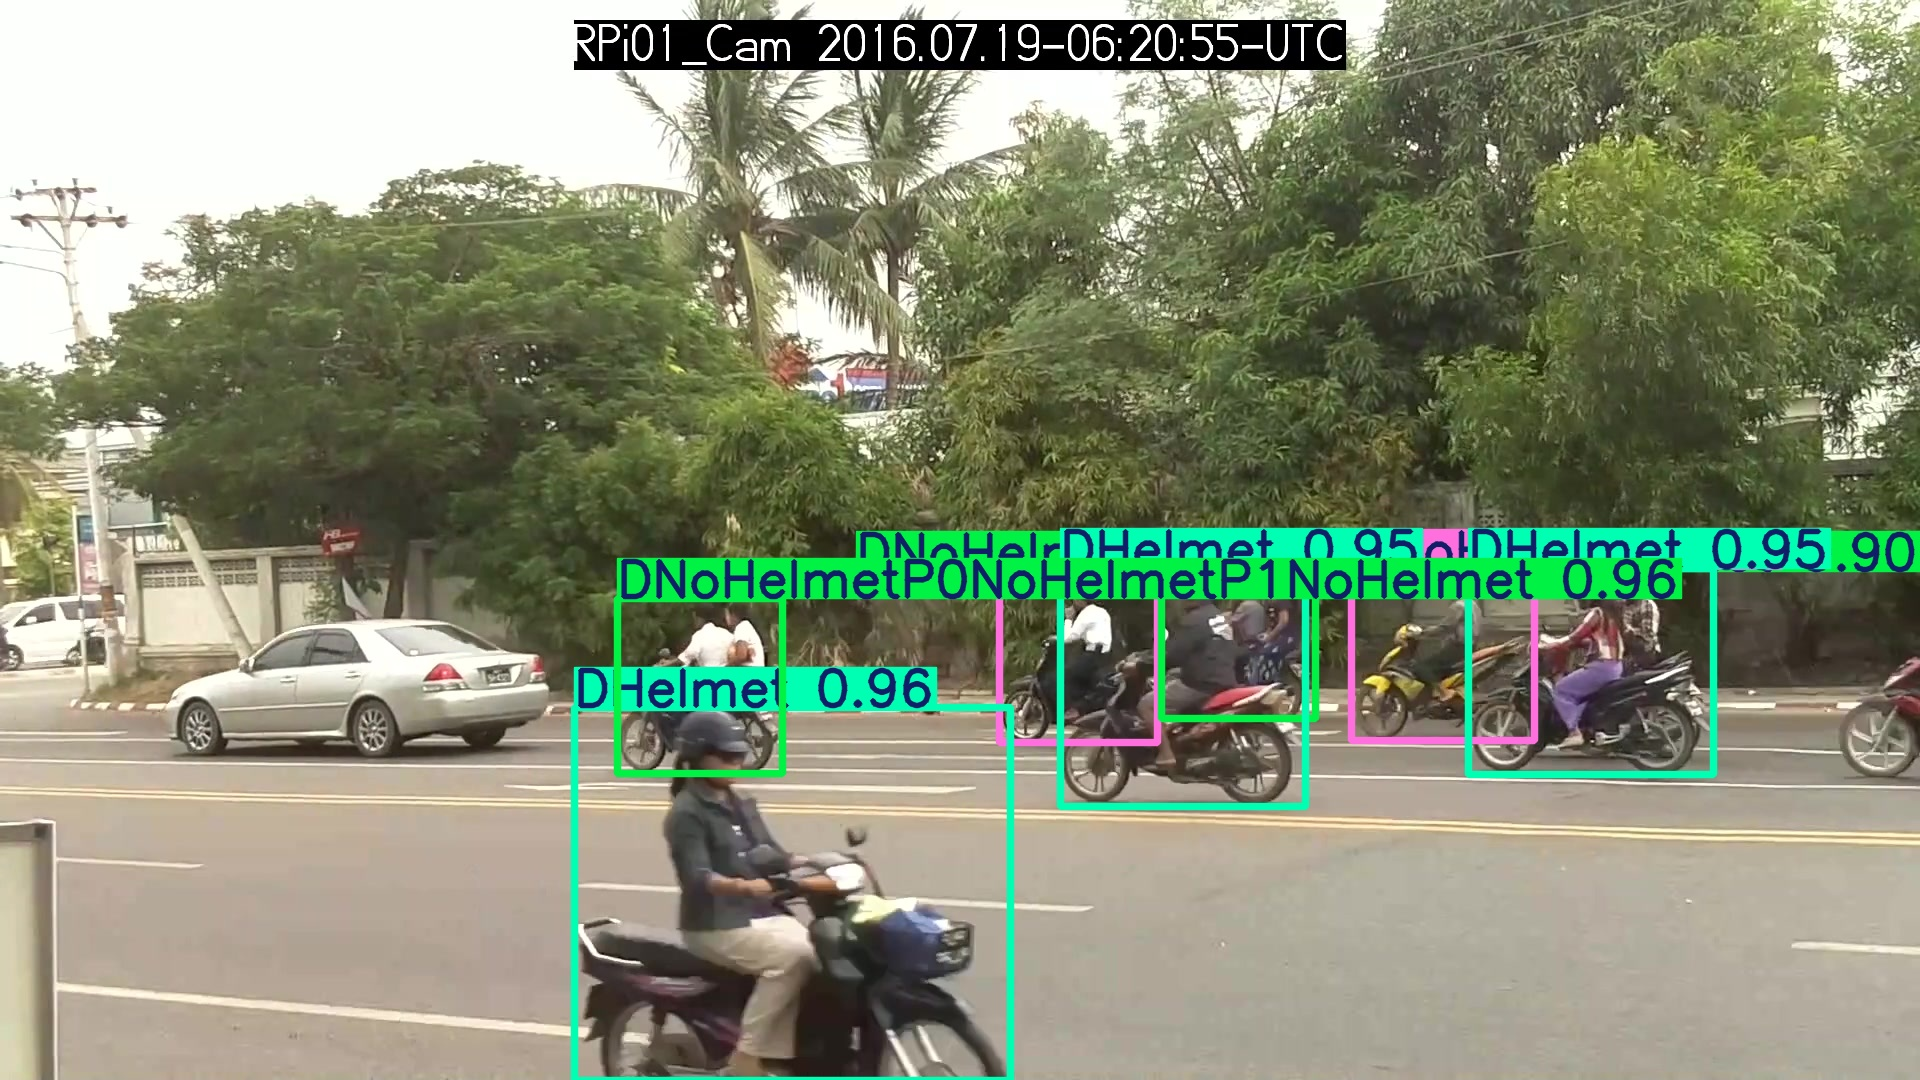
\includegraphics[width=\textwidth]{figs/chap01/result.png}
      \caption{检测结果}
      \label{fig:result}
  \end{minipage}
\end{figure}


\section{章节安排}
本文共包含六个章节,每一章的主要内容如下:

第一章:绪论。本章首先介绍了本文的研究目的与意义,对目标检测的发展历程进行概述,详细介绍了YOLO系列算法的发展过程及其在交通安全领域的应用现状,最后说明了本文的研究内容。

第二章:YOLO算法相关理论。本章主要介绍了YOLOv11算法的网络结构和损失函数。网络结构方面主要介绍主干网络、颈部网络和检测头。损失函数主要介绍边界框回归损失函数、分类损失函数和分布损失函数。最后对YOLO系列各版本的性能作了对比。

第三章:数据集构建及训练参数设置。本章介绍了本文的数据集来源以及为解决类别不平衡对数据集做的增强处理,分析了增强之后的标签数量分布情况,然后介绍了本文的实验环境和训练参数设置。

第四章:实验结果与分析。本章首先介绍了目标检测模型检测精度和速度两方面的评价指标,展示了YOLOv11n、YOLOv11s和YOLOv11m这三个模型的训练结果,对比分析了上述三个模型的精度、召回率、mAP以及检测速度,总结了各模型适用的场景。

第五章:检测系统的设计与实现。本章主要介绍了检测系统的软件设计与开发过程。从需求分析、系统架构、前端开发和后端开发这四个方面展开。

第六章:总结与展望。本章为本文的最后一张,对本文所做的工作进行总结,并展望目标检测技术在交通安全领域的未来的发展情况。
%%% Local Variables:
%%% mode: latex
%%% TeX-master: "../main.tex"
%%% End:
